\subsection{Gtransfo\-Lin  Class Reference}
\label{class_gtransfolin}\index{GtransfoLin@{Gtransfo\-Lin}}
implements the linear transformations (6 real coefficients). 


{\tt \#include $<$gtransfo.h$>$}

Inheritance diagram for Gtransfo\-Lin::\begin{figure}[H]
\begin{center}
\leavevmode
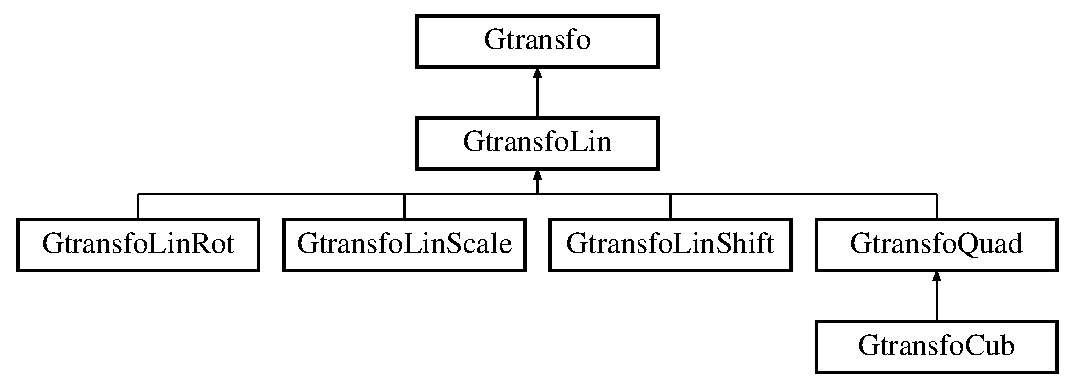
\includegraphics[height=4cm]{class_gtransfolin}
\end{center}
\end{figure}
\subsubsection*{Public Methods}
\begin{CompactItemize}
\item 
\index{GtransfoLin@{GtransfoLin}!GtransfoLin@{Gtransfo\-Lin}}\index{GtransfoLin@{GtransfoLin}!GtransfoLin@{Gtransfo\-Lin}}
{\bf Gtransfo\-Lin} ()\label{class_gtransfolin_a0}

\begin{CompactList}\small\item\em the default constructor constructs the do-nothing transformation.\item\end{CompactList}\item 
\index{operator *@{operator $\ast$}!GtransfoLin@{Gtransfo\-Lin}}\index{GtransfoLin@{GtransfoLin}!operator *@{operator $\ast$}}
Gtransfo\-Lin {\bf operator $\ast$} (const Gtransfo\-Lin \&T2) const\label{class_gtransfolin_a1}

\begin{CompactList}\small\item\em enables to combine linear tranformations: T1=T2$\ast$T3 is legal.\item\end{CompactList}\item 
\index{invert@{invert}!GtransfoLin@{Gtransfo\-Lin}}\index{GtransfoLin@{GtransfoLin}!invert@{invert}}
Gtransfo\-Lin {\bf invert} () const\label{class_gtransfolin_a2}

\begin{CompactList}\small\item\em returns the inverse: T1 = T2.invert();.\item\end{CompactList}\item 
\index{apply@{apply}!GtransfoLin@{Gtransfo\-Lin}}\index{GtransfoLin@{GtransfoLin}!apply@{apply}}
void {\bf apply} (const double Xin, const double Yin, double \&Xout, double \&Yout) const\label{class_gtransfolin_a3}

\item 
\index{Determinant@{Determinant}!GtransfoLin@{Gtransfo\-Lin}}\index{GtransfoLin@{GtransfoLin}!Determinant@{Determinant}}
double {\bf Determinant} () const\label{class_gtransfolin_a4}

\item 
void {\bf Derivative} (const {\bf Point} \&Where, Gtransfo\-Lin \&Derivative, const double Step=0.01) const
\begin{CompactList}\small\item\em Computes the local Derivative of a transfo. Step is used for numerical derivation.\item\end{CompactList}\item 
\index{LinearApproximation@{LinearApproximation}!GtransfoLin@{Gtransfo\-Lin}}\index{GtransfoLin@{GtransfoLin}!LinearApproximation@{Linear\-Approximation}}
Gtransfo\-Lin {\bf Linear\-Approximation} (const {\bf Point} \&Where, const double step=0.01) const\label{class_gtransfolin_a6}

\begin{CompactList}\small\item\em linear (local) approximation.\item\end{CompactList}\item 
\index{apply@{apply}!GtransfoLin@{Gtransfo\-Lin}}\index{GtransfoLin@{GtransfoLin}!apply@{apply}}
{\bf Point} {\bf apply} (const {\bf Point} \&Pin) const\label{class_gtransfolin_a7}

\item 
\index{dump@{dump}!GtransfoLin@{Gtransfo\-Lin}}\index{GtransfoLin@{GtransfoLin}!dump@{dump}}
void {\bf dump} (ostream \&stream=cout) const\label{class_gtransfolin_a8}

\begin{CompactList}\small\item\em dumps the transfo coefficients to stream.\item\end{CompactList}\item 
double {\bf fit} (const Star\-Match\-List \&List, const {\bf Gtransfo} $\ast$Prior\-Transfo=NULL, const {\bf Gtransfo} $\ast$Posterior\-Transfo=NULL)
\begin{CompactList}\small\item\em fits a transfo to a list of star pairs (p1,p2).\item\end{CompactList}\item 
\index{GtransfoLin@{GtransfoLin}!GtransfoLin@{Gtransfo\-Lin}}\index{GtransfoLin@{GtransfoLin}!GtransfoLin@{Gtransfo\-Lin}}
{\bf Gtransfo\-Lin} (double ox, double oy, double aa11, double aa12, double aa21, double aa22)\label{class_gtransfolin_a10}

\begin{CompactList}\small\item\em the constructor that enables to set all parameters independently. Not very useful.\item\end{CompactList}\item 
\index{GtransfoLin@{GtransfoLin}!GtransfoLin@{Gtransfo\-Lin}}\index{GtransfoLin@{GtransfoLin}!GtransfoLin@{Gtransfo\-Lin}}
{\bf Gtransfo\-Lin} (const {\bf Gtransfo\-Identity} \&T)\label{class_gtransfolin_a11}

\begin{CompactList}\small\item\em Handy converter:.\item\end{CompactList}\item 
\index{Clone@{Clone}!GtransfoLin@{Gtransfo\-Lin}}\index{GtransfoLin@{GtransfoLin}!Clone@{Clone}}
{\bf Gtransfo}$\ast$ {\bf Clone} () const\label{class_gtransfolin_a12}

\begin{CompactList}\small\item\em returns a copy (allocated by new) of the transformation.\item\end{CompactList}\item 
\index{ReduceCompo@{ReduceCompo}!GtransfoLin@{Gtransfo\-Lin}}\index{GtransfoLin@{GtransfoLin}!ReduceCompo@{Reduce\-Compo}}
{\bf Gtransfo}$\ast$ {\bf Reduce\-Compo} (const {\bf Gtransfo} $\ast$Right) const\label{class_gtransfolin_a13}

\begin{CompactList}\small\item\em allow composition of transformations regardless of their actual types.see {\bf Gtransfo\-Compose}() {\rm (p.\,\pageref{gtransfo_h_a1})} for a user callable entry.\item\end{CompactList}\item 
{\bf Gtransfo}$\ast$ {\bf Inverse\-Transfo} (const double Precision, const {\bf Frame} \&Region) const
\begin{CompactList}\small\item\em returns an inverse transfo.\item\end{CompactList}\item 
\index{A11@{A11}!GtransfoLin@{Gtransfo\-Lin}}\index{GtransfoLin@{GtransfoLin}!A11@{A11}}
double {\bf A11} () const\label{class_gtransfolin_a15}

\item 
\index{A12@{A12}!GtransfoLin@{Gtransfo\-Lin}}\index{GtransfoLin@{GtransfoLin}!A12@{A12}}
double {\bf A12} () const\label{class_gtransfolin_a16}

\item 
\index{A21@{A21}!GtransfoLin@{Gtransfo\-Lin}}\index{GtransfoLin@{GtransfoLin}!A21@{A21}}
double {\bf A21} () const\label{class_gtransfolin_a17}

\item 
\index{A22@{A22}!GtransfoLin@{Gtransfo\-Lin}}\index{GtransfoLin@{GtransfoLin}!A22@{A22}}
double {\bf A22} () const\label{class_gtransfolin_a18}

\item 
\index{dX@{dX}!GtransfoLin@{Gtransfo\-Lin}}\index{GtransfoLin@{GtransfoLin}!dX@{d\-X}}
double {\bf d\-X} () const\label{class_gtransfolin_a19}

\item 
\index{dY@{dY}!GtransfoLin@{Gtransfo\-Lin}}\index{GtransfoLin@{GtransfoLin}!dY@{d\-Y}}
double {\bf d\-Y} () const\label{class_gtransfolin_a20}

\item 
\index{Npar@{Npar}!GtransfoLin@{Gtransfo\-Lin}}\index{GtransfoLin@{GtransfoLin}!Npar@{Npar}}
virtual int {\bf Npar} () const\label{class_gtransfolin_a21}

\begin{CompactList}\small\item\em returns the number of parameters (to compute chi2's).\item\end{CompactList}\item 
\index{Degree@{Degree}!GtransfoLin@{Gtransfo\-Lin}}\index{GtransfoLin@{GtransfoLin}!Degree@{Degree}}
virtual int {\bf Degree} () const\label{class_gtransfolin_a22}

\end{CompactItemize}
\subsubsection*{Protected Methods}
\begin{CompactItemize}
\item 
\index{identity@{identity}!GtransfoLin@{Gtransfo\-Lin}}\index{GtransfoLin@{GtransfoLin}!identity@{identity}}
void {\bf identity} ()\label{class_gtransfolin_b0}

\end{CompactItemize}
\subsubsection*{Protected Attributes}
\begin{CompactItemize}
\item 
\index{dx@{dx}!GtransfoLin@{Gtransfo\-Lin}}\index{GtransfoLin@{GtransfoLin}!dx@{dx}}
double {\bf dx}\label{class_gtransfolin_n0}

\item 
\index{dy@{dy}!GtransfoLin@{Gtransfo\-Lin}}\index{GtransfoLin@{GtransfoLin}!dy@{dy}}
double {\bf dy}\label{class_gtransfolin_n1}

\item 
\index{a11@{a11}!GtransfoLin@{Gtransfo\-Lin}}\index{GtransfoLin@{GtransfoLin}!a11@{a11}}
double {\bf a11}\label{class_gtransfolin_n2}

\item 
\index{a12@{a12}!GtransfoLin@{Gtransfo\-Lin}}\index{GtransfoLin@{GtransfoLin}!a12@{a12}}
double {\bf a12}\label{class_gtransfolin_n3}

\item 
\index{a21@{a21}!GtransfoLin@{Gtransfo\-Lin}}\index{GtransfoLin@{GtransfoLin}!a21@{a21}}
double {\bf a21}\label{class_gtransfolin_n4}

\item 
\index{a22@{a22}!GtransfoLin@{Gtransfo\-Lin}}\index{GtransfoLin@{GtransfoLin}!a22@{a22}}
double {\bf a22}\label{class_gtransfolin_n5}

\end{CompactItemize}
\subsubsection*{Friends}
\begin{CompactItemize}
\item 
class {\bf Gtransfo}
\item 
class {\bf Gtransfo\-Identity}
\item 
class {\bf operator $\ast$}
\item 
class {\bf operator $\ast$}
\end{CompactItemize}


\subsubsection{Detailed Description}
implements the linear transformations (6 real coefficients).



\subsubsection{Member Function Documentation}
\index{GtransfoLin@{Gtransfo\-Lin}!Derivative@{Derivative}}
\index{Derivative@{Derivative}!GtransfoLin@{Gtransfo\-Lin}}
\paragraph{\setlength{\rightskip}{0pt plus 5cm}void Gtransfo\-Lin::Derivative (const {\bf Point} \& {\em Where}, Gtransfo\-Lin \& {\em Derivative}, const double {\em Step} = 0.01) const\hspace{0.3cm}{\tt  [virtual]}}\hfill\label{class_gtransfolin_a5}


Computes the local Derivative of a transfo. Step is used for numerical derivation.

the Derivative is represented by a Gtransfo\-Lin, in which (hopefully), the offset terms are zero. Derivative should  transform a vector of offsets into a vector of offsets. 

Reimplemented from {\bf Gtransfo} {\rm (p.\,\pageref{class_gtransfo_a9})}.

Reimplemented in {\bf Gtransfo\-Quad} {\rm (p.\,\pageref{class_gtransfoquad_a9})}.\index{GtransfoLin@{Gtransfo\-Lin}!InverseTransfo@{InverseTransfo}}
\index{InverseTransfo@{InverseTransfo}!GtransfoLin@{Gtransfo\-Lin}}
\paragraph{\setlength{\rightskip}{0pt plus 5cm}{\bf Gtransfo}$\ast$ Gtransfo\-Lin::Inverse\-Transfo (const double {\em Precision}, const {\bf Frame} \& {\em Region}) const\hspace{0.3cm}{\tt  [virtual]}}\hfill\label{class_gtransfolin_a14}


returns an inverse transfo.

Precision and Region refer to the \char`\"{}input\char`\"{} side of this,  and hence to the output side of the returned {\bf Gtransfo} {\rm (p.\,\pageref{class_gtransfo})}. 

Reimplemented from {\bf Gtransfo} {\rm (p.\,\pageref{class_gtransfo_a12})}.

Reimplemented in {\bf Gtransfo\-Quad} {\rm (p.\,\pageref{class_gtransfoquad_a8})}.\index{GtransfoLin@{Gtransfo\-Lin}!fit@{fit}}
\index{fit@{fit}!GtransfoLin@{Gtransfo\-Lin}}
\paragraph{\setlength{\rightskip}{0pt plus 5cm}double Gtransfo\-Lin::fit (const Star\-Match\-List \& {\em List}, const {\bf Gtransfo} $\ast$ {\em Prior\-Transfo} = NULL, const {\bf Gtransfo} $\ast$ {\em Posterior\-Transfo} = NULL)\hspace{0.3cm}{\tt  [virtual]}}\hfill\label{class_gtransfolin_a9}


fits a transfo to a list of star pairs (p1,p2).

After the fit this(Prior\-Transfo(p1)) yields approximately Posterior\-Transfo(p2). The returned value is the chi2. 

Reimplemented from {\bf Gtransfo} {\rm (p.\,\pageref{class_gtransfo_a4})}.

Reimplemented in {\bf Gtransfo\-Lin\-Shift} {\rm (p.\,\pageref{class_gtransfolinshift_a2})}, {\bf Gtransfo\-Lin\-Rot} {\rm (p.\,\pageref{class_gtransfolinrot_a2})}, {\bf Gtransfo\-Quad} {\rm (p.\,\pageref{class_gtransfoquad_a5})}, and {\bf Gtransfo\-Cub} {\rm (p.\,\pageref{class_gtransfocub_a6})}.

The documentation for this class was generated from the following file:\begin{CompactItemize}
\item 
{\bf gtransfo.h}\end{CompactItemize}
